
La figure ci-dessous représente une pièce de bois qui est un parallélépipède rectangle de
longueur 10, de largeur 5 et de hauteur 3.

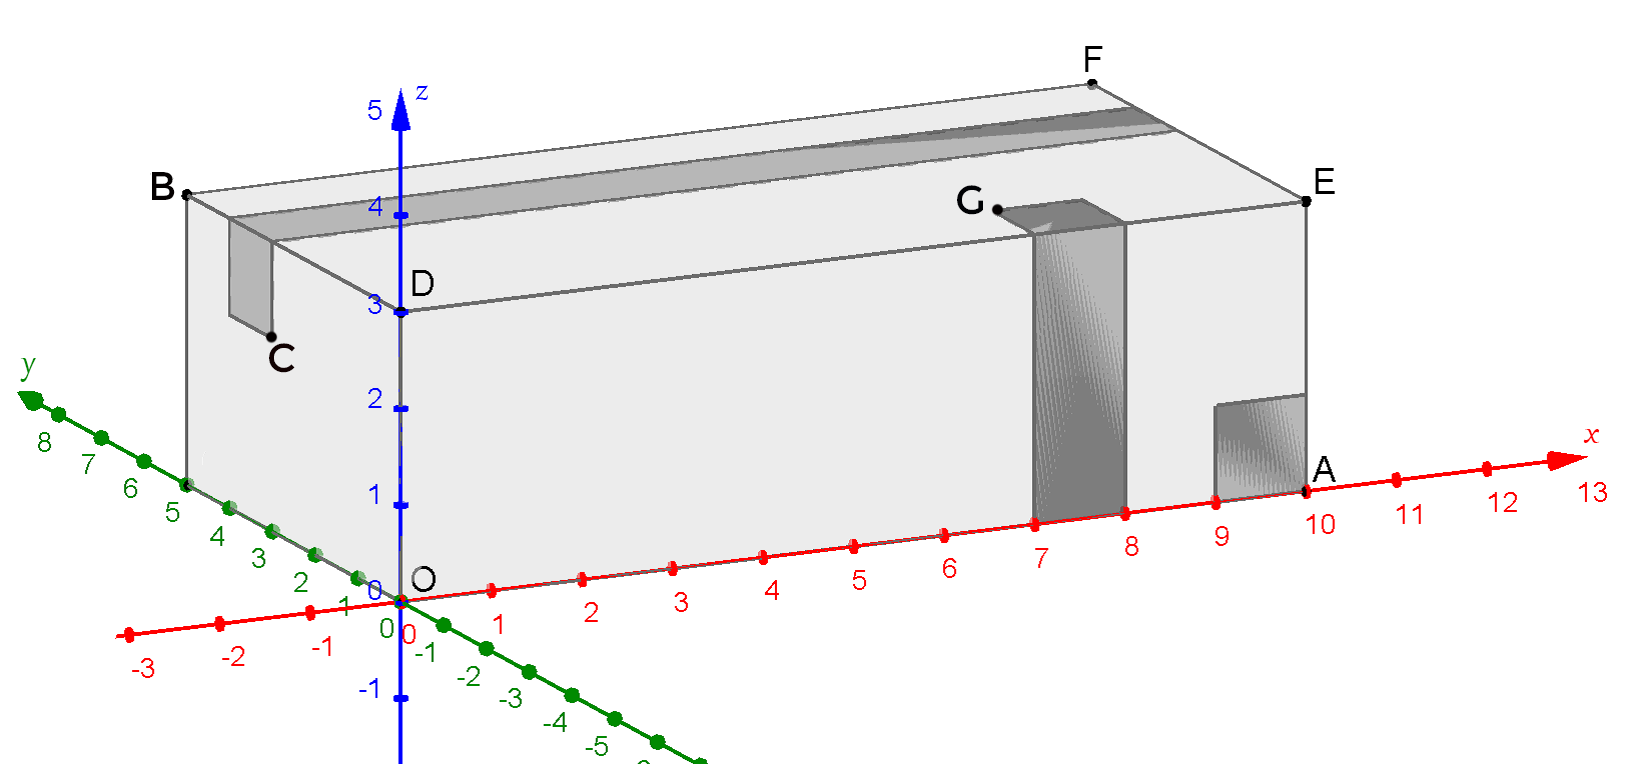
\includegraphics[scale=0.25]{RepE-parallelepipedecoordonnees.png}\\ 

L’espace est repéré à l’aide d’un repère d’origine O (visible sur la figure) : dans ce repère, les
points A, C et D ont pour coordonnées : $A (10 ; 0 ; 0)$, $C (0 ; 5 ; 0)$ et $D (0 ; 0 ; 3)$.\\

On crée un nouveau solide en retirant les trois parallélépipèdes rectangles dessinées sur la
figure : les bases de ces parallélépipèdes sont des carrés de côté 1.

\medskip

Représenter une vue de face, une vue de côté et une vue de dessus de ce nouveau solide.
%Donner les coordonnées (abscisse, ordonnée, altitude) de tous les sommets visibles sur ces
%différentes vues de ce nouveau solide.

